\chapter{Media Item Deduplication}
\label{cha:media-item-deduplication}

% the code below specifies where the figures are stored
\ifpdf
    \graphicspath{{7_media_item_deduplication/figures/PNG/}{7_media_item_deduplication/figures/PDF/}{7_media_item_deduplication/figures/}}
\else
    \graphicspath{{7_media_item_deduplication/figures/EPS/}{7_media_item_deduplication/figures/}}
\fi

\section{Introduction}

In \autoref{cha:media-item-extraction},
we have motivated the need for media item deduplication.
By clustering media items, we get a~higher-level view on
a~media item cluster's overall performance on different networks.
As detailed in \autoref{sec:definition}, media items can be
photos or videos.
WordNet~\cite{fellbaum1998wordnet,miller1995wordnet} defines
the term \emph{duplicate} as
\textit{``a copy that corresponds to an original exactly''}.
The corresponding verb \emph{to duplicate} is defined as to
\textit{``make a~duplicate or duplicates of''}.
The derived term \emph{deduplication} in consequence refers to
the act of eliminating duplicate or redundant information.

In this chapter, we will treat video
and photo deduplication separately. 
Our goal is to deduplicate media items \emph{on-the-fly}
at the very moment they are extracted from social networks.
Due to this limitation, we cannot rely on any preprocessing
that state-of-the-art algorithms rely on.
Our approaches to video and photo near-duplicate
and exact duplicate detection are founded
on a~tile-wise histogram-based pixel comparison algorithm.

\subsection{Definitions}

We have defined a~social media item as either a~photo (image) or video
that was \emph{publicly} shared or published
on at least one social network.
In the following, we will use the shorter term media item
rather than the full term and define
what we mean with \emph{duplicate media items} for various cases.

\paragraph{Exact Duplicates for Photos:}

We define two media items of type photo as \emph{exact duplicates}
if their pixel contents are exactly the same.
This implies that by our definition a~scaled or recompressed version
of the same photo is \emph{not} considered an exact duplicate. 
Similarly, a~rotated version of a~photo is also \emph{not}
considered an exact duplicate. 
In contrast, two photo files with different file names
or different Exchangeable image file
format\footnote{\url{http://www.cipa.jp/english/hyoujunka/kikaku/pdf/DC-008-2010_E.pdf},
accessed July 15, 2013}
(Exif) data are considered exact duplicate
if their pixel contents are exactly the same.
Exact duplicate photos typically occur if users share content 
from one social network on another, for example,
if one user posts a~photo on Instagram that then someone else
(or even the same user) posts on Facebook.

\paragraph{Near-Duplicates for Photos:}

We define two media items of type photo as \emph{near-duplicates}
if their pixel contents differ no more than a~given threshold after resampling.
Examples of near-duplicate photos are scaled versions
of the same photo, photos shot from a~slightly different angle,
rotated photos up to a~certain degree, \emph{etc.}
Near-duplicate photos typically occur if event attendants
stand close to each other and thus take photos
from a~similar standpoint.
Another scenario is when a~user applyies a~photo effect to a~photo
(like an Instagram filter) and then shares both the modified
and the unmodified version.

\paragraph{Duplicates for Videos:}

We define two media items of type video as \emph{exact duplicates}
if their pixel contents are frame by frame exactly the same.
In practice, we lower this condition and instead of every frame
only consider frames at shot boundaries.
We make \emph{no} requirements on the audio, \emph{i.e.},
a~video that has been dubbed in two different languages,
but that fulfills the pixel contents equality condition,
is considered exact duplicate.
Typical scenarios where exact duplicate videos can occur is,
for example, two users sharing the same YouTube video
independently from each other.

\paragraph{Near-Duplicates for Videos:}

We define two media items of type video as \emph{near-duplicates}
if their pixel contents per frame differ no more
than a~given threshold.
In practice, we lower this condition and instead of every frame
only consider frames at shot boundaries.
Typical scenarios where near-duplicate videos can occur is through
logo or subtitle insertion, resizing, re-encoding,
or aspect-ration changes.
Note that we do not consider video subsegments near-duplicates.

\paragraph{Special Case of Photo Contained in a~Video:}

We define the special case of
\emph{a photo being contained in a~video} if the pixel contents
of a~photo media item differ no more than a~given threshold from
the pixel contents of any of the frames of a~video media item.
In practice, we lower this condition and instead of every frame
only consider frames at shot boundaries.
Typically, this phenomenon occurs if two event attendants
of the same event both cover it from almost the same
standpoint, however, if the one attendant takes a~video,
while the other attendant takes a~photo.

\section{Related Work}

Related work in the field of media item deduplication
and clustering can be separated in different areas,
which reflects the grouping of our definitions above.
We further show related work on media fragments,
digital storytelling, and Natural Language Generation,
which we combine for a~novel algorithm debugging approach.

\paragraph{Image Deduplication and Clustering:}

Work on ordinal measures that serve as a~general tool for
image matching was performed by Bhat \emph{et~al.}\
in~\cite{bhat1998imagecorrespondence}.
Chum \emph{et~al.}\ have proposed a~near-duplicate image detection method
using MinHash and term frequency-inverse document frequency (tf-idf)
weighting~\cite{chum2008nearduplicate}.
They use a~visual vocabulary of vector quantized local feature descriptors based on
Scale-Invariant Feature Transform (SIFT)~\cite{lowe1999sift}.
Gao \emph{et~al.}\ \cite{gao2005webimageclustering} have proposed an image clustering method
in the context of Web image clustering, which clusters images
based on the consistent fusion of the information contained in
both low-level features and surrounding texts.
Also in the context of Web pages, Cai
\emph{et~al.}\ \cite{cai2004hierarchicalclustering} have proposed
a~hierarchical clustering method using visual, textual, and link analysis.
Goldberger \emph{et~al.}\ \cite{goldberger2006unsupervisedclustering} 
have combined discrete and continuous image models based on a~mixture of Gaussian densities
with a~generalized version of the information bottleneck principle
for unsupervised hierarchical image set clustering. 
Chen \emph{et~al.}\ \cite{chen2003cbir} have introduced an image retrieval approach,
which tackles the semantic gap problem by learning similarities
of images of the same semantics.

\paragraph{Video Deduplication and Clustering:}

Specialized methods for video deduplication exist,
for example~\cite{min2011nearduplicatevideo,wu2009nearduplicate}
by Min \emph{et~al.}\ who, given the observation that 
transformations tend to preserve the semantic information conveyed
by the video content, propose an approach for identifying
near-duplicate videos by making use of both low-level visual
features and high-level semantic features
detected using trained classifiers.
In~\cite{oliveira2010nearduplicate}, Oliveira
\emph{et~al.}\ report on four large-scale online surveys
wherein they have confirmed that humans perceive videos as near-duplicates
based on both non-semantic features like different image or audio
quality, but also based on semantic features like different
videos of similar content.
A~survey of video deduplication methods has been conducted by
Lian \emph{et~al.}\ in~\cite{lian2010survey}.
In~\cite{guil2007clustering}, Guil \emph{et~al.}\ have proposed a~method
for detecting copies of a~query video in a~videos database
that groups frames with similar visual content while maintaining their temporal order.
In~\cite{okamoto2002videoclustering}, Okamoto \emph{et~al.}\  have proposed an approach
that is based on fixed length video stream segments.
By generating spatio-temporal images, they employ co-occurrence matrices
to express features in the time dimension explicitly. 
Yi \emph{et~al.}\ have proposed motion histograms~\cite{yi2005motionhistogram},
where the motion content of a~video at pixel level is represented
as a~Pixel Change Ratio Map (PCRM), which captures the motion intensity,
spatial location, and size of moving objects in a~video sequence. 

\paragraph{Image \emph{and} Video Deduplication and Clustering:}

A~method for both images \emph{and} videos
has been proposed by Yang \emph{et~al.}\ \cite{yang2009nearduplicate}.
The authors describe a~system for detecting duplicate images and videos
in a~large collection of multimedia data that uses local difference patterns
as the unified feature to describe both images and videos.
It has been demonstrated that the proposed method is robust against
common image-processing tasks used to produce duplicates.

\paragraph{Media Fragments:}

There are many online video hosting platforms
that have some sort of media fragments support.
In the following, we present two representative ones.
The video hosting platform YouTube%
\footnote{YouTube: \url{http://www.youtube.com/}}
allows for deep-linking into videos
via a~proprietary URL parameter \texttt{t},
whose value has to match the regular expression
\texttt{\textbackslash d+m\textbackslash d+s} (for minutes and seconds),
as documented in~\cite{youtube2008link}.
Dailymotion\footnote{Dailymotion: \url{http://www.dailymotion.com/}}
has similar URL parameters \texttt{start} and \texttt{end},
whose values have to match the regular expression
\texttt{\textbackslash d+} (for seconds).
The CSS Backgrounds and Borders Module Level~3 specification%
~\cite{bos2012css3} defines the \texttt{background-size} property
that can be used to crop media items visually
and thus create the illusion of a~spatial media fragment
when combined with a~wrapping element.
Media Fragments URI~\cite{troncy2012mediafragments}
specifies a~syntax for constructing media fragments URIs
and explains how to handle them
when used over the HTTP protocol~\cite{fielding1999http}.
The syntax is based on the specification of particular name-value pairs
that can be used in URI query strings and URI fragment identifiers
to restrict a~media resource to a~certain fragment.
The temporal and spatial dimensions are currently supported
in the basic version of Media Fragments URIs.
Combinations of dimensions are also possible.

\paragraph{Digital Storytelling:}

Pizzi and Cavazza report in~\cite{pizzi2008debugging}
on the development of an authoring technology
on top of an interactive storytelling system
that originated as a~debugging%
\footnote{Pizzi and Cavazza use the term \emph{debugging}
in the non-IT sense: to check for redundancy, dead-ends, consistency, \emph{etc.}\ in
authored stories} tool for a~planning system.
Alexander and Levine define in~\cite{alexander2008storytelling}
the term \emph{Web~2.0 storytelling},
where people create \emph{microcontent}---%
small chunks of content, with each chunk conveying a~primary idea---%
that gets combined with social media to form coherent stories.
We use Media Fragments URIs to help human annotators
understand the results of an algorithm
by converting dry software debugging data to digital stories.

\paragraph{Natural Language Generation:}

Natural language generation is the natural language processing task
of generating natural language from a~machine representation system.
This field is covered in great detail by Reiter and Dale
in~\cite{reiter2000building}.
They divide the task into three stages:
document planning, microplanning, and realization.
\emph{Document planning} determines the content and structure of a~document.
\emph{Microplanning} decides which words, syntactic structures,
\emph{etc.}\ are used to communicate the chosen content and structure.
\emph{Realization} maps the abstract representations
used by microplanning into text.

\section{Photo Deduplication}
\label{sec:photo-deduplication}

We determine the popularity of media items
shared across social networks.
This task involves the deduplication of extracted media items.
In \autoref{cha:shot-boundary-detection}, we have presented an algorithm
for on-the-fly shot boundary detection for video media items.
In this chapter, we will show how components of this algorithm
can be used to deduplicate photos.

\subsection{Problem Statement}
\label{sec:problem-statement}

Our work is situated in the broader context of summarizing events
based on social network data.
In order to get an overview of a~given event based on a~\emph{potentially large} set
of event-related media items, this set of media items needs to be \emph{pruned}
to exclusively contain highly relevant media items that are as representative
for the event as possible.
Rather than showing the viewer all media items,
clusters of similar media items need to be formed.
Within each cluster, the most representative media item
has to be decided on according to well-defined criteria.
Undesired duplicate or near-duplicate content in the context of social networks
arises in a~number of situations
that we will illustrate in the following.

\subsubsection{Duplicate Content}
\label{sec:duplicate-content}

Duplicate content in the context of social networks
arises whenever people either share exactly the same,
or an exact copy of a~given media item.
An example of the latter can be one user uploading the same media item
to the two different social networks \googleplus and Facebook.
An example of the prior can be two users sharing the same
YouTube video independently from each other, or re-sharing each other's content.

\subsection{Near-Duplicate Content}
\label{sec:near-duplicate-content}

Near-duplicate content in the context of social networks
arises in a~number of situations
that we will illustrate in the following.
All photos are real examples of media items shared on social networks
that were clustered correctly as near-duplicates
by our clustering algorithm, which we will detail in
\autoref{sec:near-duplicate-clustering-algorithm}.

\paragraph{Different Viewing Angle:}

When two people attend the same event
and create media items at roughly the same time
covering the same scene,
their media items will be similar
and---the capturing devices' quality aside---only differ in the viewing angles. 
\autoref{fig:viewing-angle} shows a~concrete example.

\begin{figure}[!h]
  \centering
  \subfloat[Viewing angle 1]{
    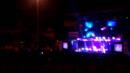
\includegraphics[height=2.7cm]{stage1.jpg}
  }                
  \subfloat[Viewing angle 2]{
    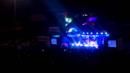
\includegraphics[height=2.7cm]{stage2.jpg}
  }
  \caption{Slightly different viewing angles of a~concert stage}
  \label{fig:viewing-angle}  
\end{figure}

\paragraph{Logo, Watermark, Lower Third, or Caption Insertion:}

Oftentimes, organizations or individuals insert
logos, watermarks, lower thirds, or captions into media items
to highlight their origin, to convey related information,
or to claim ownership of a~media item.
An example of caption, logo, and lower third insertion
can be seen in \autoref{fig:logo}.

\begin{figure}[!h]
  \centering
  \subfloat[Blank]{
    
\includegraphics[width=0.26\textwidth]{speaker1.jpg}
  }                
  \subfloat[Caption]{
    
\includegraphics[width=0.26\textwidth]{speaker2.jpg}
  }
  \subfloat[Logo, lower third]{
    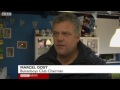
\includegraphics[width=0.26\textwidth]{speaker3.jpg}
  }
  \caption{Caption, logo, and lower third insertion for a~speaker}
  \label{fig:logo}  
\end{figure}

\paragraph{Cropping:}

Cropping refers to the removal of the outer parts of a~media item
to improve framing, accentuate subject matter,
or to (lossily) change the aspect ratio.
Cropping either happens manually via an image editing application
or, more often, by the social networks themselves
to obtain a~square aspect ratio
that better fits the timeline view of users,
as can be seen in the example in \autoref{fig:cropping}.

\begin{figure}[!h]
  \centering
  \subfloat[Original]{
    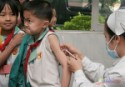
\includegraphics[height=3cm]{kid1.jpg}
  }                
  \subfloat[Cropped]{
    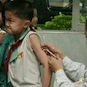
\includegraphics[height=3cm]{kid2.jpg}
  }
  \caption[Original and cropped version of a~photo]
  {Original and cropped version of a~photo (including a~slight color variation)}
  \label{fig:cropping}  
\end{figure}

\paragraph{Different Keyframes:}

We have shown an approach to camera shot boundary detection
in \autoref{cha:shot-boundary-detection} and~\cite{steiner2012shotdetection}.
Different frames stemming from the same camera shot
can occur on social networks when preview heuristics
attempt to auto-select a~representative poster frame from a~video with different approaches,
typically resulting in varying frames for different social networks.
\autoref{fig:camera-shot} shows an example of this phenomenon.

\begin{figure}[!h]
  \centering
  \subfloat[Frame 1]{
    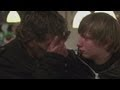
\includegraphics[height=3cm]{camera1.jpg}
  }                
  \subfloat[Frame 2]{
    
\includegraphics[height=3cm]{camera2.jpg}
  }
  \caption[Two different frames stemming from the same camera shot]
    {Two different frames stemming from the same camera shot,
    with the left frame appearing slightly earlier in the video}
  \label{fig:camera-shot}  
\end{figure}

\paragraph{Aspect Ratio Changes with Squeezing or Stretching:}

Aspect ratio changes can either happen combined with cropping
(and thus losing parts of the media item) and/or combined with 
squeezing or stretching (and thus deforming the media item).
\autoref{fig:bulged} shows an example where a~media item gets stretched.

\begin{figure}[!h]
  \centering
  \subfloat[Original]{
    
\includegraphics[height=3cm]{lordoftherings.jpg}
  }                
  \subfloat[Stretched]{
    
\includegraphics[height=3cm]{lordoftheringsstretched.jpg}
  }
  \caption{Original and stretched version of a~photo}
  \label{fig:bulged}  
\end{figure}

\paragraph{Photo Filters:}

With the raising popularity of Instagram with its 90 million monthly active users,%
\footnote{\url{http://instagram.com/press/}, accessed July 15, 2013}
photo filters that, \emph{e.g.}, emulate retro Polaroid\texttrademark\ or tilt-shift effects
are a~considerable reason for near-duplicate media content on social networks.
\autoref{fig:photo-filter} shows a~typical example.

\begin{figure}[!h]
  \centering
  \subfloat[Original]{
    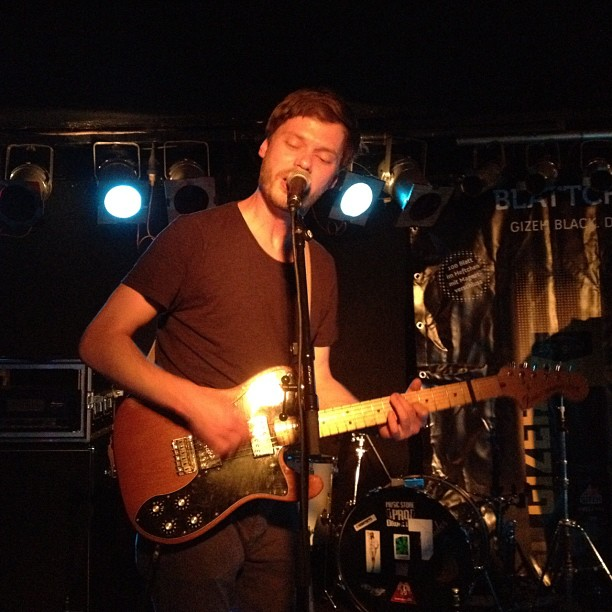
\includegraphics[width=0.25\textwidth]{clickclickdecker1.jpg}
  }                
  \subfloat[With photo filter]{
    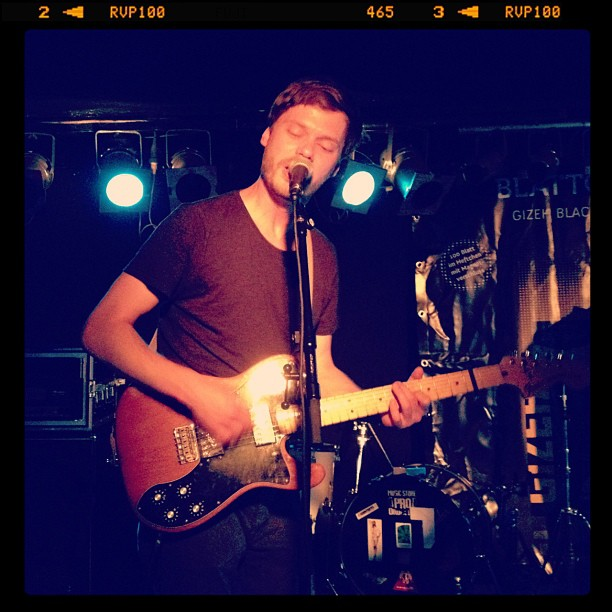
\includegraphics[width=0.25\textwidth]{clickclickdecker2.jpg}
  }
  \caption{Original and version with an applied photo filter of a~photo}
  \label{fig:photo-filter}  
\end{figure}

\subsection{Near-Duplicate Photo Clustering Algorithm}
\label{sec:near-duplicate-clustering-algorithm}

In the previous section, we have outlined
reasons and sources for duplicate and near-duplicate content.
In this section, we describe an algorithm tailored to
deduplicating and clustering exact-duplicate and near-duplicate media items.
Design goals for the algorithm include
the capability to detect exact-duplicate and near-duplicate media items
in a~timely, entirely \emph{ad hoc} manner without any pre-calculation.
In general---and especially for big events---event coverage on social networks
is very broad, \emph{i.e.}, there exist more media items
than one could consume in a~reasonable time.
In consequence, it is tolerable for the algorithm to cluster media items aggressively
rather than leaving too many media items unclustered.
The algorithm has a~twofold approach to clustering:
\emph{low-level} analysis by looking at tile-wise pixel data,
combined with \emph{high-level} analysis by detecting faces in media items.
In the following, we describe the face detection component
of our media item clustering algorithm.

\subsection{Face Detection}
\label{sec:face-detection}

Face detection is a~computer vision technology
that determines the regions of faces in media items.
Rotation-invariant face detection aims to detect faces with arbitrary
rotation angles and is crucial as the first step in automatic face detection
for general applications, as face images on social media are seldom upright and frontal.
Face detection is a~subclass of the broader class of object detection.
The Viola-Jones object detection framework proposed in 2001
by Paul Viola and Michael
Jones~\cite{viola2001objectdetection,viola2004facedetection}
provides competitive object detection rates in realtime
and was motivated primarily by the problem of face detection.
We use an algorithm that further improves Viola-Jones,
based on work by Huang \emph{et~al.}\ \cite{huang2007facedetection}
and Abramson \emph{et~al.}\ \cite{abramson2007yef}
in a~JavaScript implementation made available by Liu~\cite{liu2012facedetection}.
This algorithm is fast enough to be applied to hundreds of media items
in well less than a~second overall processing time on a~standard laptop
(mid-2010 MacBook~Pro).

\subsection{Algorithm Description}

Our near-duplicate media item clustering algorithm belongs to the family of
tile-wise histogram-based clustering algorithms.
As an additional semantic feature, the algorithm considers detected faces
as described above.
For two media items to be clustered,
the following conditions have to be fulfilled.

\begin{enumerate}
  \item Out of $m$ tiles of a~media item with $n$ tiles ($m \leq n$),
    at most $\textit{tiles\_threshold}$ tiles may differ not more than $\textit{similarity\_threshold}$
    from their counterpart~tiles.
  \item The numbers $f_1$ and $f_2$ of detected faces in both media items
    have to be the same.
    We note that we do not \emph{recognize} faces, but only \emph{detect} them.
\end{enumerate}

The algorithm pseudocode can be seen in \autoref{code:clustering}.
In the actual implementation some speed improvements,
for example, looking up already calculated
distances\footnote{\texttt{distances[outerItem][innerItem] =
distances[innerItem][outerItem]}}
have been applied;
these were omitted in the listing for legibility reasons.
We calculate the histograms and distances only once initially.
The clusters are then recalculated dynamically
whenever either $\textit{tiles\_threshold}$ or $\textit{similarity\_threshold}$ change.
The given values of $\textit{rows} = \textit{cols} = 10$ and
$\textit{tiles\_threshold} = 67 = \lceil \textit{rows} \cdot \textit{cols} \cdot 2/3 \rceil$
and $\textit{similarity\_threshold} = 15$ were determined empirically
on a~large corpus of event-related media items
and are known to deliver solid results.
The corpus has been made available publicly,
see \autoref{sec:evaluation-chpater6} for the details.

\begin{lstlisting}[,caption={[Simplified pseudocode of the deduplication and clustering algorithm]{Simplified pseudocode of the exact- and near-duplicate
  media item deduplication and clustering algorithm}},
  label={code:clustering},escapechar=§]
§\textbf{Input:}§ mediaItems, a~list of media items
§\textbf{Output:}§ clusters, a~list of clustered media items

§\textbf{init:}§


§\textit{\# Algorithm settings}§
ROWS = 10
COLS = 10
TILES_THRESHOLD = ceil(ROWS * COLS * 2/3)
SIMILARITY_THRESHOLD = 10


§\textit{\# Calculates tile-wise histograms}§
histograms = {}
faces = {}
§\textbf{for}§ item §\textbf{in}§ mediaItems
  faces[item] = getFaces(item)
  
  histograms[item] = {}
  §\textbf{for}§ tile §\textbf{in}§ item
    histograms[item][tile] = getHistogram(tile)
  §\textbf{end for}§
§\textbf{end for}§  

    
§\textit{\# Calculates tile-wise distances}§
distances = {}
§\textbf{for}§ outerItem §\textbf{in}§ mediaItems
  distances[outerItem] = {}
  §\textbf{for}§ innerItem §\textbf{in}§ mediaItems
    distances[outerItem][innerItem] = {}
    §\textbf{for}§ tile §\textbf{in}§ histograms[outerItem]
      distances[outerItem][innerItem][tile] =
          abs(histograms[outerItem][tile] -
              histograms[innerItem][tile])
    §\textbf{end for}§
  §\textbf{end for}§
§\textbf{end for}§

  
§\textit{\# Calculates clusters}§
clusters = {}
§\textbf{for}§ outerItem §\textbf{in}§ mediaItems  
  clusters[outerItem] = []  
  §\textbf{for}§ innerItem §\textbf{in}§ mediaItems
    §\textbf{if}§ outerItem == innerItem §\textbf{then}§ continue
    
    similarTiles = 0
    distance = distances[outerItem][innerItem]
    §\textbf{for}§ tile §\textbf{in}§ distance      
      §\textbf{if}§ distance[tile] <= SIMILARITY_THRESHOLD §\textbf{then}§
        similarTiles++
      §\textbf{end if}§
    §\textbf{end for}§
         
    §\textit{\# Check condition 1 (tiles)}§
    §\textbf{if}§ similarTiles >= TILES_THRESHOLD §\textbf{then}§
      §\textit{\# Check condition 2 (faces)}§
      §\textbf{if}§ faces[outerItem] == faces[innerItem] §\textbf{then}§
        clusters[outerItem].push(innerItem)
      §\textbf{end if}§
    §\textbf{end if}§    
  §\textbf{end for}§
§\textbf{end for}§

§\textbf{return}§ clusters        
\end{lstlisting}

\subsection{Experiments}

We have evaluated the near-duplicate photo clustering
on two events from (at time of writing) recent history with high social network coverage
that we will briefly describe in the following.

\paragraph{Grammy Awards Nominations 2013:}

The Grammy Award---or short Grammy---is an award by
the National Academy of Recording Arts and Sciences of the United States
to recognize outstanding achievement in the music industry.
The annual ceremony features performances by prominent artists.
Some of the awards are presented in a~widely viewed televised ceremony.
On December 5, 2012, the nominees for the 55\superscript{th} Annual Grammy Awards
were announced at an event broadcasted live by CBS
titled \emph{Grammy Nominations Concert
Live},\footnote{\url{http://en.wikipedia.org/wiki/2013_Grammy_Awards},
accessed July 15, 2013}
during which Taylor Swift and LL~Cool~J revealed the nominees
in several key categories, including the so-called Big Four:
Album, Record and Song of the Year, and Best New Artist.
CBS suggested the hashtag \texttt{\#GRAMMYNoms} for the event.

\paragraph{Victoria's Secret Fashion Show 2012:}
\label{sec:vsfashionshow}

The \emph{Victoria's Secret Fashion
Show}\footnote{\url{http://en.wikipedia.org/wiki/Victoria's_Secret_Fashion_Show},
accessed July 15, 2013} is an annual event
sponsored by Victoria's Secret, a~brand of lingerie and sleepwear.
The show features some of the world's leading fashion models
and is used by the brand to promote and market its goods in high-profile settings.
American network television broadcasts the show during prime time.
The show is a~lavish event with elaborate costumed lingerie and
varying music by leading entertainers
that attracts hundreds of celebrities and entertainers,
with special performers and acts every year.
The 2012 edition of the show,
which was previously taped on November 7, 2012
was aired on December 4, 2012 on CBS
to an audience of 9.48 million viewers.
CBS suggested the hashtag \texttt{\#VSFashionShow} for the event.

\subsection{Evaluation}\label{sec:evaluation-chpater6}

We have collected and made available%
\footnote{\url{https://www.dropbox.com/sh/2llvjaut32juwrx/7eGLodfP_2},
accessed July 15, 2013}
datasets for both events with
379 photos for the \emph{Victoria's Secret Fashion Show 2012} event 
and 949 photos for the \emph{Grammy Awards Nominations 2013} event.
These photos were collected using the media item extraction framework
described in \autoref{cha:media-item-extraction}
using a~mix of hashtag searches with the official event hashtags combined
with full-text searches for event titles and variations thereof~%
\cite{becker2010eventidentification,becker2012plannedevents}.
Due to the short-lived nature of social networks,
the returned results of the media item extraction process itself
are not reproducible.
Additionally, our focus in this chapter
is on media item deduplication and clustering, not extraction.
The concrete clustering parameters for the algorithm were set as listed below.

\begin{enumerate}
  \item $\textit{rows}$ = $\textit{cols}$ = $10$
  \item $\textit{tiles\_threshold}$ = $67$
  \item $\textit{similarity\_threshold}$ = $15$
\end{enumerate}

In the following, we discuss the clustering and deduplication results.
\autoref{fig:topvsfashionshow} and \autoref{fig:topgrammy} show the top clusters
for the \emph{Victoria's Secret Fashion Show 2012} and the 
\emph{Grammy Awards Nominations 2013} events respectively.
We then pick some representative examples from both events
and have a~closer look at the clustering algorithm's strengths and weaknesses.

\begin{figure}[!h]
  \centering
  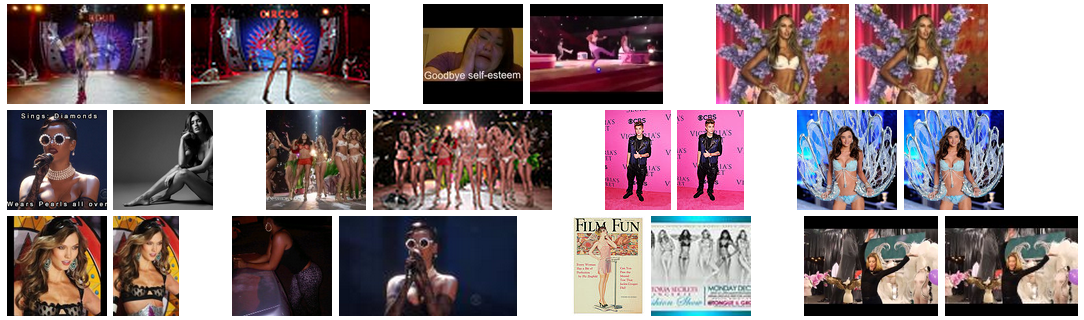
\includegraphics[width=1.0\linewidth]{./vsfashionshow_clusters.png}
  \caption{Top clusters for the \emph{Victoria's Secret Fashion Show 2012} event}
  \label{fig:topvsfashionshow}
\end{figure}

\begin{figure}[!h]
  \centering
  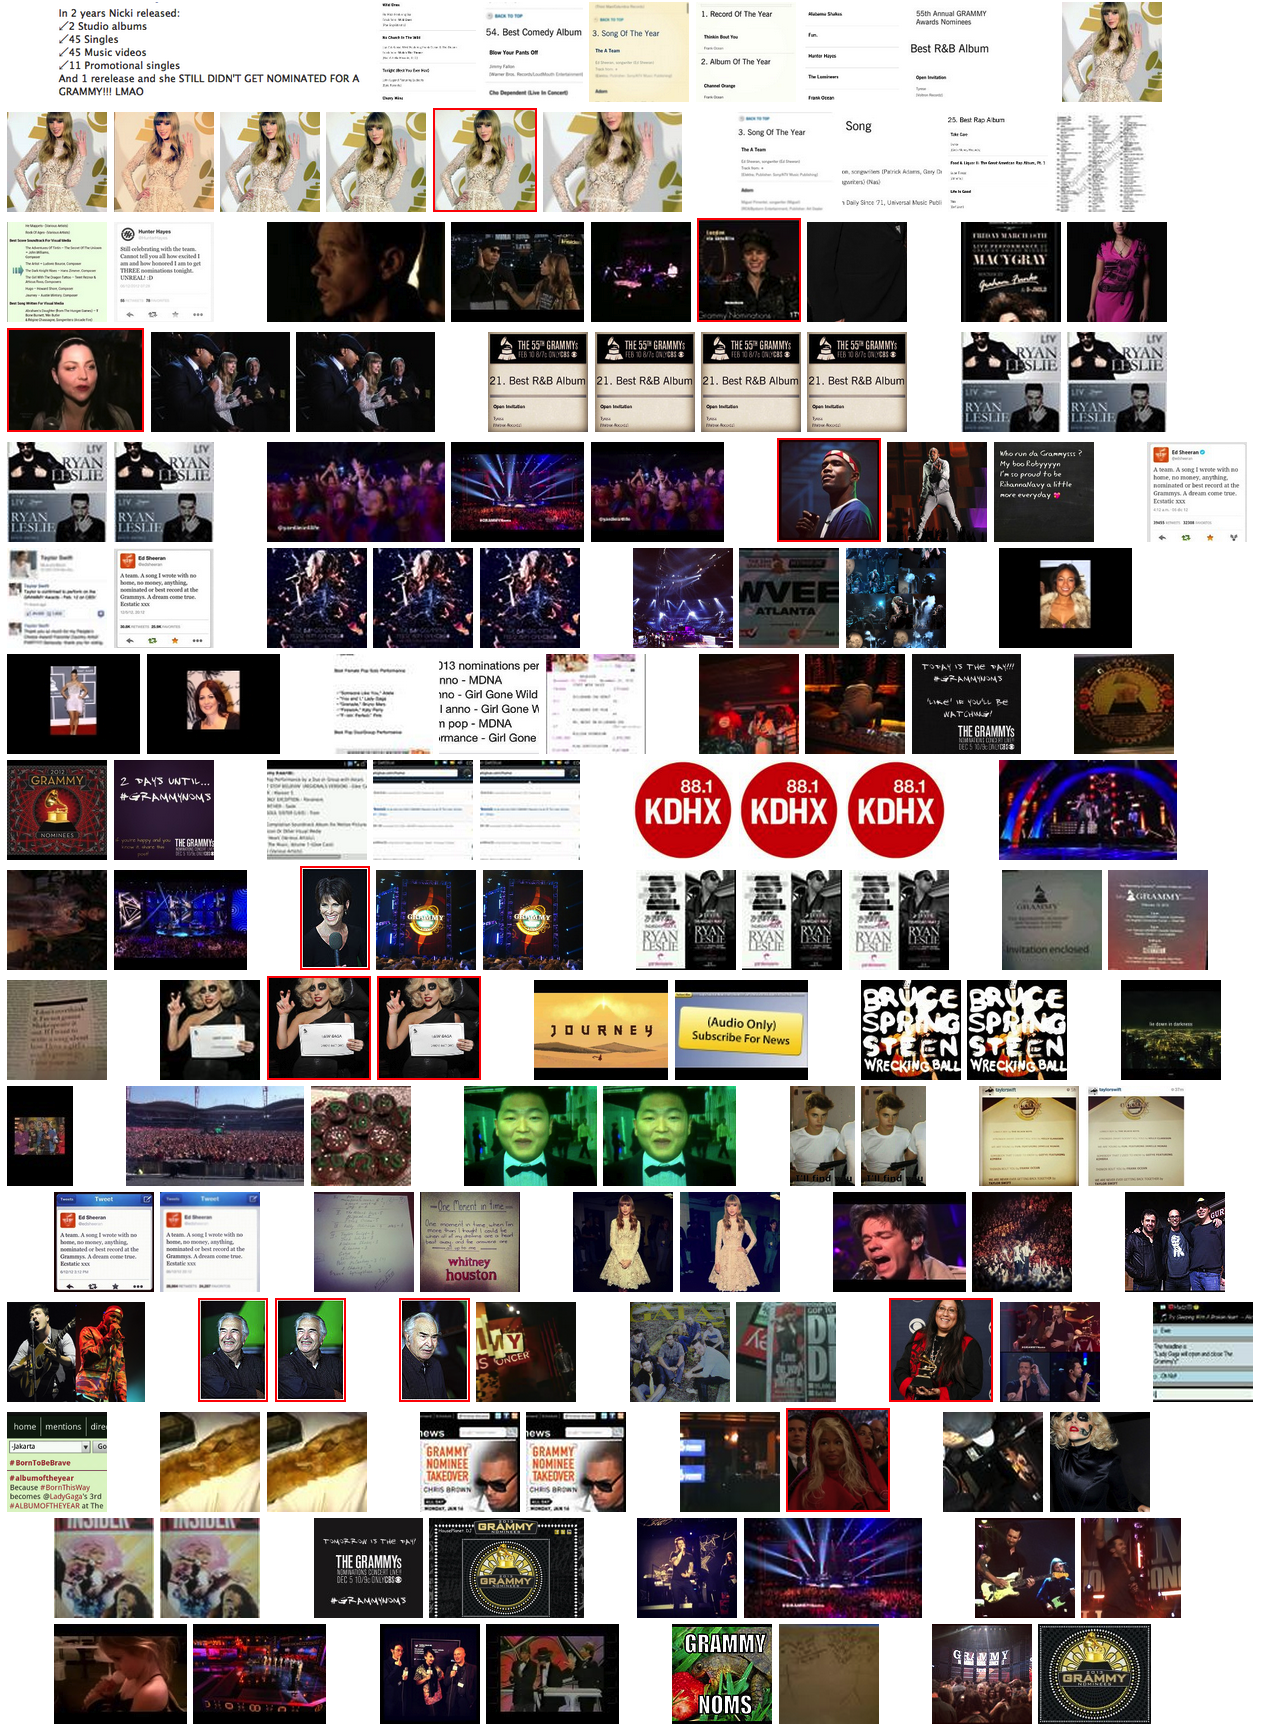
\includegraphics[width=0.95\textwidth,height=0.9\textheight,keepaspectratio]{./grammy_clusters.png}
  \caption{Top clusters for the \emph{Grammy Awards Nominations 2013} event}
  \label{fig:topgrammy}
\end{figure}

\paragraph{Algorithm Strengths:} 

\autoref{fig:personclose} has a~brunette fashion model in a~pink robe
and a~heart-shaped pink spotlight as central elements of both photos. 
Even though the model is shot from different angles and at different times,
the photos are successfully clustered due to the very identifying colors
and the high tile-wise similarity. 

\begin{figure}[!h]
  \centering
  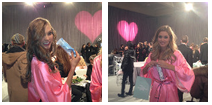
\includegraphics[width=0.4\linewidth]{./person.png}
  \caption{High tile-wise similarity of a~dominating color}
  \label{fig:personclose}
\end{figure}

\autoref{fig:scenecrop} shows two different views of a~stage
taken at slightly different times.
The left photo covers a~detail of the scene,
whereas the right photo covers the entire stage.
Due to the high tile-wise similarity of the scene detail,
the photos are successfully clustered.

\begin{figure}[!h]
  \centering
  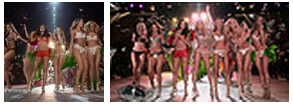
\includegraphics[width=0.5\linewidth]{./scene.png}
  \caption{Cropped view of a~stage scene}
  \label{fig:scenecrop}
\end{figure}

\autoref{fig:lightingconditions} shows two views of a~stage
under different lighting conditions.
Due to the tile color tolerances and the high tile-wise similarity,
the photos are successfully clustered.

\begin{figure}[!h]
  \centering
  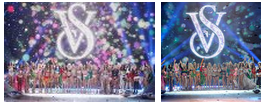
\includegraphics[width=0.5\linewidth]{./viewing_angle.png}
  \caption{Stage and detail of a~stage under different lighting conditions}
  \label{fig:lightingconditions}
\end{figure}

\autoref{fig:zoomed} shows two photos of the same fashion model,
where the left photo is a~zoomed version of the right photo 
with added black bars so that the resulting photo
has a~square aspect ratio.
Despite the differences, the photos are successfully clustered.

\begin{figure}[!h]
  \centering
  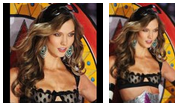
\includegraphics[width=0.35\linewidth]{./zoom.png}
  \caption{Zoomed view of a~model with black bars left and right}
  \label{fig:zoomed}
\end{figure}

\autoref{fig:stageperson} shows two views of the same stage,
however, with a~different person.
Due to the dominating tile-wise similarity of the stage tiles,
the photos are correctly clustered.

\begin{figure}[!h]
  \centering
  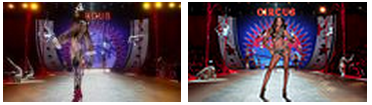
\includegraphics[width=0.6\linewidth]{./stage.png}
  \caption{Two views of the same stage with different person}
  \label{fig:stageperson}
\end{figure}

\paragraph{Algorithm Weaknesses:}

\autoref{fig:white} shows five media items with pure white
as the dominating color and a~pure black font
stemming from screenshots of the Grammy results from Web pages.
The algorithm in its previously described form clusters such media items.
This may or may not be desired.

\begin{figure}[!h]
  \centering
  
\includegraphics[width=1\linewidth]{./white.png}
  \caption[Pure white as dominating color stemming from screenshots]
    {Pure white as dominating color stemming from screenshots
    (bad quality caused by down-scaling via the originating social networks)}
  \label{fig:white}
\end{figure}

Likewise, at the other end of the color spectrum,
\autoref{fig:bwtolerance} shows two media items of a~woman
with pure black as the dominating color,
one time with and the other time without added black bars
to fit a~letterbox aspect ratio.
In its previously described form, the algorithm
does \emph{not} cluster such media items
(unless a~very small number $\textit{tiles\_threshold}$ 
of required similar tiles is selected).
In the majority of cases, though, clustering such media items \emph{is} desired.
Our response to both issues is to ignore a~certain part
of the color spectrum in the algorithm's similarity measure.
In the concrete case, ignoring pure white and pure black correctly fixed
the clustering in our chosen example events in all but one cases,
without negatively impacting previously correctly formed clusters.

\begin{figure}[!h]
  \centering
  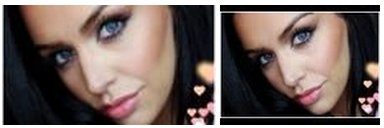
\includegraphics[width=0.55\linewidth]{./bwtolerance.png}
  \caption[Black bars added to fit a~16:9 image in a~4:3 letterbox]
    {Black bars added to fit a~16:9 image in a~4:3 letterbox
    (the white border is part of the original photo)}
  \label{fig:bwtolerance}
\end{figure}

Finally, \autoref{fig:weakness} shows two entirely different media items
that were incorrectly clustered as the tile histograms
were similar enough under the chosen similarity threshold.
The explanation for this is twofold.
First, the original source media items were very small thumbnail-like images,
which hindered face recognition
(there is actually an \emph{unequal} number of faces in each image).
Second, the way the algorithm works
causes the tiles of very tiny media items like the ones in question to blur.

\begin{figure}[!h]
  \centering
  
\includegraphics[width=0.4\linewidth]{./weakness.png}
  \caption{Entirely different photos with similar tile histograms}
  \label{fig:weakness}
\end{figure}

We have experienced in our experiments that there is no single perfect
combination of algorithm parameters,
so the only way to address this issue (besides ignoring too small media items,
which in practice might be the easiest and best solution)
is to make the parameters flexible.
In our graphical user interface, we have created sliders
that let the user interactively preview clustering changes.
As noted before, a~screenshot of the application
is available online at the URL \url{http://twitpic.com/c02qfs/full} (accessed July 15, 2013).

\section{Video Deduplication}

In the previous section, we have introduced
an algorithm for photo deduplication.
In the upcoming section, we will outline the conceptual framework
of how this algorithm can be combined with the previously introduced
video shot boundary detection algorithm from \autoref{cha:shot-boundary-detection}.
This will allows us to on the one hand
directly deduplicate videos on a~shot boundary frame basis
or on the other hand to detect
whether a~given photo is contained in a~video.

\subsection{Photo-contained-in-Video Workflow}

In a~first step, for a~given video, we detect shot boundaries
as described before in \autoref{sec:videoshotboundarydetection}.
To illustrate this,
\autoref{fig:vsfashionshowboundaries} shows an excerpt
of detected shot boundaries for a~video related to
the \emph{Victoria's Secret Fashion Show 2012} event.
The first photo of each shot boundary film stripe
is selected as the particular shot's representative photo.
To detect whether a~given photo stemming from social networks
is contained in the video in question,
the set of extracted shot representative photos is compared
with all social network photos,
some of which are shown in \autoref{fig:topvsfashionshow}.
We note, however, that especially for longer videos
(about 4 minutes and longer)
this approach does not scale due to the sheer number of camera shots
in common videos shared on social networks,
which causes the process to consume too much time in practice.
At the expense of exactness, (the few) poster still frames
that are typically returned by video hosting platform APIs
can be used rather than extracting (all) shot boundaries manually.

\begin{figure}[!h]
  \centering
  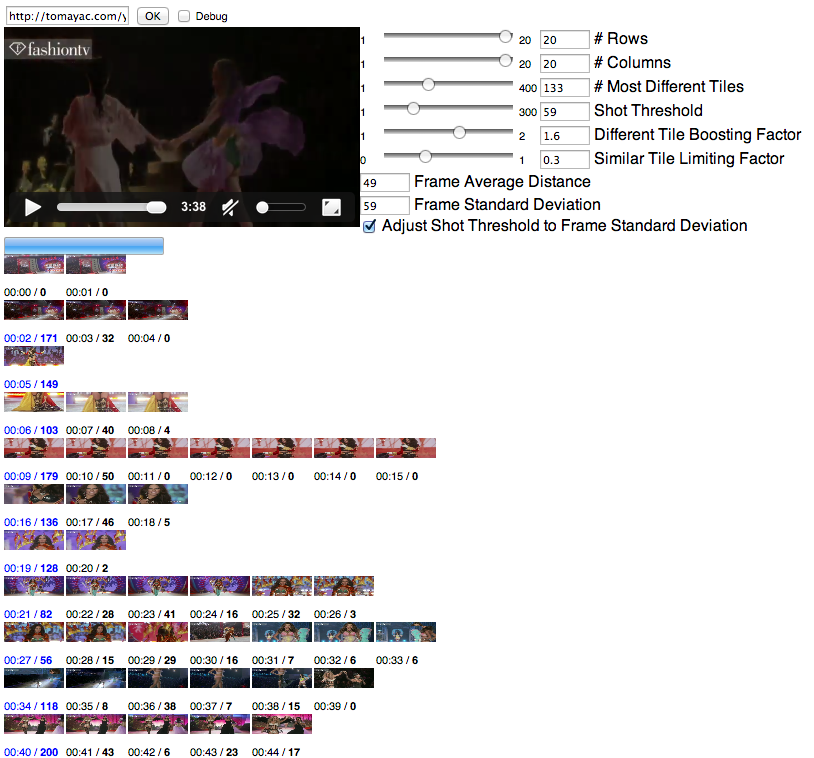
\includegraphics[width=1.0\linewidth]{./vsfashionshowboundaries.png}
  \caption[Excerpt of detected shot boundaries in an event video]
  {Excerpt of detected shot boundaries in a~\emph{Victoria's Secret Fashion Show 2012} event video}
  \label{fig:vsfashionshowboundaries}
\end{figure}

\subsection{Video-contained-in-Video Workflow}

To detect whether a~given video is contained in another,
we follow a~similar approach as outlined in the previous subsection,
with the sole difference being that we need to compare
all detected shot boundary representative photos of the source video
with the ones from the other.
Naturally, this approach is even less scalable
with regard to system response time.
The practicable work-around is, as before, to limit oneself
to poster frames delivered by the video hosting platforms.
Our experiments have shown that this approach works very well
for common social network user behavior.
For example, the 3:19 minutes long video of Mark Zuckerberg explaining
the design and engineering challenges behind Facebook's
recently announced Graph Search product was initially published
on Facebook,\footnote{\url{https://www.facebook.com/about/graphsearch},
accessed July 15, 2013} however, people republished the same video 
multiple times on YouTube.
As the YouTube-generated poster frames were similar enough
and even if the other video metadata like title and description
were different, we were able to effectively deduplicate the videos
with the described work-around approach.

\section{Describing Media Item Differences with Media Fragments URI and Speech Synthesis}

In this section, we describe how media item differences
can be described with media fragments URIs and speech synthesis.
We will combine the two techniques for the purpose of
introducing a~novel algorithm debugging approach,
illustrated with our previously described
media item clustering algorithm.

\subsection{Algorithm Debug View}
\label{sec:algorithm-debug-view}

In order to illustrate the way the algorithm clusters media items,
\autoref{fig:algorithmdebugtwoclusters} shows a~debug view of the algorithm
for two clustered media items related to the 
\emph{Grammy Awards Nominations 2013} event.
The red border around the media item indicates at least one detected face.
Independent from the actual media item's aspect ratio,
the tile-wise comparison always happens based on a~potentially squeezed
square aspect ratio version.
The two slightly different media items (caption insertion, lighting change)
were clustered, because out of the $10 \cdot 10 = 100$ tiles,
$85$ of the minimum required $\textit{tiles\_threshold}$ of $67$ tiles differed not more
than the $\textit{similarity\_threshold}$ of $15$ per tile.
In both media items, exactly $1$ face was detected.
A~screenshot of the complete media item clustering application (with a~different event)
is available online at \url{http://twitpic.com/c02qfs/full} (accessed July 15, 2013).

\begin{figure}[!h]
  \centering
  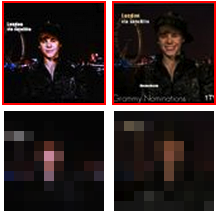
\includegraphics[width=0.5\linewidth]{./algorithmdebug.png}
  \caption[Algorithm debug view for two clustered media items]
  {Algorithm debug view for two clustered media items
  related to the \emph{Grammy Awards Nominations 2013} event
  (the red border around the media items indicates at least one detected face)}
  \label{fig:algorithmdebugtwoclusters}
\end{figure}

\subsection{Media Fragments Requirements}
\label{sec:media-fragment-requirements}

A~media fragment is a~part that was separated from its parent media item.
In order to make statements about such media fragments,
we need to uniquely identify them.
In the context of our research on media item deduplication and clustering,
media fragments identifiers need to be capable of expressing the following concepts.

\begin{enumerate}
  \itemsep0em
  \item Given a~rectangular media item with the dimensions
    $ width \times height $, express that in turn rectangular
    tiles of smaller dimensions are part of the original media item.
  \item Given detected faces at the granularity level of bounding rectangles,
    express that these bounding rectangles are within the dimensions
    of the original media item and that each bounding rectangle contains a~face.
  \item Requirements \textit{i} and \textit{ii} need to be fulfilled
    for both types of media items, \emph{i.e.}, photos and videos. In case of the latter,
    video subsegments of any length---including video still frames---need to be supported.
\end{enumerate}

Media Fragments URI~\cite{troncy2012mediafragments}
as described in the basic version of the specification
supports all three requirements.
The \emph{temporal dimension} is denoted by the parameter name \texttt{t}
and specified as an interval with a~begin time and an end time.
Either one or both parameters may be omitted,
with the begin time defaulting to 0 seconds
and the end time defaulting to the duration of the source media item.
The interval is half-open: the begin time is considered part of the interval,
whereas the end time is considered to be the first time point
that is not part of the interval.
If only a~single value is present, it corresponds to the begin time,
except for when it is preceded by a~comma,
which indicates the end time.
The temporal dimension is specified as Normal Play Time
(NPT,~\cite{schulzrinne1998realtime}).

The \emph{spatial dimension} selects an area of pixels from media items.
In the current version of the specification,
only rectangular selections are supported.
Rectangles can be specified as pixel coordinates or percentages.
Rectangle selection is denoted by the parameter name \texttt{xywh}.
The value is either \texttt{pixel:} or \texttt{percent:}
(defaulting to \texttt{pixel:}) and four comma-separated integers.
The integers denote $x$, $y$, $width$, and $height$ respectively,
with $x = 0$ and $y = 0$ being the top left corner of the media item.
If \texttt{percent:} is used,
$x$ and $width$ are interpreted as a~percentage of the width of the original media item,
while $y$ and $height$ are interpreted as a~percentage of the original height.
While (at time of writing) the temporal dimension is implemented natively
in common Web browsers, this is not the case for the spatial dimension.

The intent of the Ontology for Media Resources~\cite{lee2012mediaontology}
by Lee \emph{et~al.}\ is to bridge different description methods of media resources
and to provide a~core set of descriptive properties.
Combined with Media Fragments URI, this allows for making statements
about media items and fragments thereof.
An example in RDF Turtle syntax~\cite{prudhommeaux2013turtle}
is given in \autoref{code:media-fragment}.

\begin{lstlisting}[caption={[Description of two 10~sec long media fragments]{Description of two 10~sec long media fragments:
  \textit{(i)}~a~tile of dimensions $ 30 \times 40 $ pixels
  starting at pixel coordinates $ (0, 0) $
  that contains a~face; and
  \textit{(ii)}~a~tile of dimensions $ 10 \times 10 $ pixels
  starting at pixel coordinates $ (0, 0) $ of red color}},
  label=code:media-fragment, float=!h]
@base <http://example.org/> .
@prefix ma: <http://www.w3.org/ns/ma-ont> .
@prefix foaf: <http://xmlns.com/foaf/0.1/> .
@prefix db: <http://dbpedia.org/resource/> .
@prefix dbo: <http://dbpedia.org/ontology/> .
@prefix col: <http://purl.org/colors/rgb/> .

<video> a ma:MediaResource .
<video#t=,10&xywh=0,0,30,40> a ma:MediaFragment ;
                             foaf:depicts db:Face .
<video#t=,10&xywh=0,0,10,10> a ma:MediaFragment ;
                             dbo:colour col:f00 .
\end{lstlisting}

\subsection{Algorithm Debug Properties}
\label{sec:media-item-deduplication-algorithm}

The deduplication algorithm described in this chapter
belongs to the family of tile-wise histogram-based clustering algorithms.
As an additional semantic feature, the algorithm considers detected faces.
It is capable of deduplicating media items of type video and/or photo.
In the case of video, frames at camera shot boundaries are used.
To illustrate the algorithm debugging mechanics,
we use a running example of two media items related to a~music video by the 
band Backstreet Boys, which can be seen in \autoref{fig:near-duplicate}.
For media items to be clustered,
the following clustering conditions have to be fulfilled.

\begin{description}
  \itemsep0em
  \item[Cond.~1] Out of $m$ tiles of a~media item with $n$ tiles ($m \leq n$),
    the average color of at most $\textit{tiles\_threshold}$ tiles
    may differ not more than $\textit{similarity\_threshold}$
    from their counterpart tiles.
  \item[Cond.~2] The numbers $f_1$ and $f_2$ of detected faces
    in both media items have to be the same.
    We note that the algorithm does not \emph{recognize} faces,
    but only \emph{detects} them.
  \item[Cond.~3] If the average colors of a~tile and its counterpart tile
    are within the black-and-white tolerance $\textit{bw\_tolerance}$,
    these tiles are not considered and $\textit{tiles\_threshold}$
    is decreased accordingly (we will talk about $\textit{effective\_tiles\_threshold}$
    in \autoref{sec:debugging-the-algorithm}).
\end{description}

The black-and-white tolerance $\textit{bw\_tolerance}$ avoids media items
to be clustered when the particular tiles are too dark (\emph{e.g.},
for the video borders in \autoref{fig:near-duplicate}) or too bright (\emph{e.g.},
for screenshots of Web pages or applications, which frequently appear on social networks).
In order to illustrate the way the algorithm deduplicates media items,
\autoref{fig:algorithmdebugtilesimilarity} shows a~debug view of the algorithm
for the two clustered media items related to the previous example
around the \emph{Backstreet Boys} music video.
Independent of the actual media items' aspect ratios,
the tile-wise comparison always happens based on
a~potentially squeezed square aspect ratio version.

\begin{figure}[!h]
  \centering
  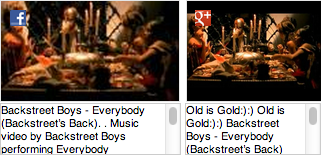
\includegraphics[width=0.9\linewidth]{./backstreetboys.png}
  \caption[\emph{Near-duplicate} music video \emph{Everybody} by the \emph{Backstreet Boys}]{\emph{Near-duplicate} music video \emph{Everybody} by the \emph{Backstreet Boys} shared independently on Facebook and \googleplus}
  \label{fig:near-duplicate}
\end{figure}

\begin{figure}[!h]
  \centering
  \subfloat[From Facebook user]{
    
\includegraphics[width=0.35\linewidth]{debug1.png}
  }
  \subfloat[From Google+ user]{
    
\includegraphics[width=0.35\linewidth]{debug2.png}
  }
  \caption[Debug view of the media item deduplication algorithm]{Debug view of the media item deduplication algorithm:
  since no faces are detected in \autoref{fig:near-duplicate},
  the clustering is based on tile similarity;
  pure black tiles are not considered due to the chosen black-and-white tolerance)}
  \label{fig:algorithmdebugtilesimilarity}
\end{figure}

\subsubsection{Debugging the Algorithm}
\label{sec:debugging-the-algorithm}

In this subsection, we consider the following three debug scenarios
that occurred most frequently during our previous experiments with human raters.
They correspond to situations where, given a~set of
deduplicated and clustered media items, a~human annotator wanted
to understand the specific details leading to the decisions
taken by the algorithm that they were unsure about or had decided on differently.

\begin{description}
  \itemsep0em
  \item[Clustering Consent.] Two or more media items are clustered
    by the algorithm and the human rater agrees.
    The human rater wants to understand why they were clustered.
  \item[Clustering Dissent.] Two or more media items are clustered
    by the algorithm, but the human rater thinks
    that they should not have been clustered.
    The human rater wants to understand why they were incorrectly clustered.
  \item[Non-Clustering Dissent.] Two or more media items are not clustered
  by the algorithm, but the human rater thinks
  that they should have been clustered.
  The human rater wants to understand why they were not clustered.
\end{description}

In order to provide answers to these human raters' information needs,
different levels of the algorithm's internals have to be debugged.
Is the $\textit{tiles\_threshold}$ (\emph{i.e.},
the number of tiles that may differ) too high or too low?
Complementary to this, is the $\textit{similarity\_threshold}$
(\emph{i.e.}, the maximum amount two tiles may differ)
too high or too low (\textbf{Cond.~1})?
Are the number of detected faces $f_1$ and $f_2$ the same?
Are all faces correctly detected, or should the face matching condition
be temporarily disregarded, \emph{e.g.}, with too tiny media items,
where faces fail to be detected (\textbf{Cond.~2})?
If the media items to be compared have very dark and/or very bright parts,
is the $\textit{bw\_tolerance}$ too high or too low (\textbf{Cond.~3})?

\subsubsection{Low-Level Debug Output}
\label{sec:low-level-debug-output}

As a~consequence of the previous observations, the low-level debug output
must include the currently selected $\textit{tiles\_threshold}$ and
$\textit{similarity\_threshold}$ and how many tiles with the present algorithm settings
currently fulfill \textbf{Cond.~1}.
In addition to that, the debug output has to contain
the number of detected faces $f_1$ and $f_2$ in each media item,
\emph{i.e.}, whether \textbf{Cond.~2} is fulfilled,
as well as the number of not considered tiles
(according to $\textit{bw\_tolerance}$), which implies fulfillment of \textbf{Cond.~3}
and potentially impacts \textbf{Cond.~1} in form of
the $\textit{effective\_tiles\_threshold}$.
For instance, the low-level debug output for the media items
from the running example of the \emph{Backstreet Boys} media items
for the music video \emph{Everybody} reads as follows.

\begin{verbatim}
- Similarity threshold: 15 (Cond. 1)
- Tiles threshold: 67 (Cond. 1)
- Similar tiles: 52 (Cond. 1)
- Faces left: 0. Faces right: 0 (Cond. 2)
- BW tolerance: 1 (Cond. 3)
- Not considered tiles: 22 (Cond. 3)
- Effective tiles threshold: 45 (Cond. 3)
\end{verbatim}

While this low-level debug output is sufficient to respond
to the polar question (yes/no question) whether media items
are clustered at all or not, it does not help with
the non-polar \emph{why} question
(the linguistic term for this type of questions is \emph{wh–question}).
In the following subsection, we show how
this low-level debug output can be lifted.

\subsection{From Debug Output to Story}
\label{sec:from-debug-output-to-story}

In order for human raters to get answers to the question on
\emph{why} media items are clustered, we need to lift the low-level debug output
to a~high-level natural language story for
the previously defined debug scenarios \textit{Clustering Consent},
\textit{Clustering Dissent}, and \textit{Non-Clustering Dissent}.
This results in a~natural language generation task,
whose three stages according to Reiter's and Dale's
architecture~\cite{reiter2000building} will be detailed in the following.

\subsubsection{Generating Natural Language}
\label{sec:text-to-speech-espeak}

\paragraph{Document Planning:}

In our context, the document is a~set of low-level debug data
as illustrated in \autoref{sec:low-level-debug-output}.
The natural language generation task is thus manageable.
We need to convey the currently selected $\textit{tiles\_threshold}$
and $\textit{similarity\_threshold}$, the number of detected faces
$f_1$ and $f_2$ in each media item, and the number of tiles
not considered given the $\textit{bw\_tolerance}$ parameter.

\paragraph{Microplanning:}

The microplanning task is driven by the debug scenarios
that were described previously.
Initially, we need to decide on a~matching condition aspect
of the algorithm that will be first highlighted.
Typically, this will be the overall tiles statistics.
Afterwards, we need to elaborate on secondary matching conditions
such as detected faces and black-and-white tolerance.
The grammatical number (plural or singular)
needs to be taken into account when statements about tile(s) or face(s)
are planned. Some values, \emph{e.g.},
the percentage of matching tiles, are calculated.
The microplanner needs to decide when exactness
(\emph{e.g.},~\textit{``99\% of all tiles''})
and when approximation of calculated values
(\emph{e.g.}, \textit{``roughly 50\%''}) better suits
the human evaluators' information needs. Neutral non-judgmental statements
(\emph{e.g.}, \textit{``45 tiles''}) and biased judgmental statements
(\emph{e.g.}, \textit{``not a~single one [tile]''})
need to be carefully balanced. Finally, in the interest of
a~more naturally sounding phrase composition,
the microplanner needs to be aware of contrasting juxtaposition
(\emph{e.g.}, \textit{``Both the left and the right media item
contain one detected face.''} \emph{vs.}
\textit{``The left media item contains no detected faces,
while the right media item contains one detected face.''}).

\paragraph{Realization:}

We show examples of sentences that are actually generated
for the three different debug scenarios (Quotes~1--3).
For the sake of completeness, we provide one additional example
(Quote~4) for the debug scenario \textbf{Non-Clustering Consent}.
The running example of the \emph{Backstreet Boys} media items
for the music video \emph{Everybody} is represented by Quote~1.

\begin{description}
  \itemsep0em
  \item[Clustering Consent] (Quote~1). \textit{``The two media items
    are near-duplicates. Out of overall 100 tiles,
    52 from the minimum required 45 tiles
    were similar enough to be clustered. This corresponds to 52 percent
    of all tiles. However, 22 tiles were not considered,
    as they are either too bright or too dark,
    which is a~common source of clustering issues.
    Neither the left, nor the right media item contain detected faces.''}
  \item[Clustering Dissent] (Quote~2). \textit{``The two media items
    are near-duplicates. Out of overall 100 tiles,
    41 from the minimum required 41 tiles were similar enough to be clustered.
    This corresponds to 41 percent of all tiles.
    However, 26 tiles were not considered, as they are either too bright
    or too dark, which is a~common source of clustering issues.
    Neither the left, nor the right media item contain detected faces.''}
  \item[Non-Clustering Dissent] (Quote~3). \textit{``The two media items
    are different. Out of overall 100 tiles,
    only 8 from the minimum required 67 tiles
    were similar enough to be clustered. This corresponds to 8 percent of all tiles.
    The left media item contains 2 detected faces,
    while the right media item contains 1 detected face.''}
  \item[(Non-Clustering Consent)] (Quote~4). \textit{``The two media items
    are different. Out of overall 100 tiles, not a~single one
    was similar enough to be clustered. Neither the left,
    nor the right media item contain detected faces.''}
\end{description}

\subsubsection{Technical Implementation}

\paragraph{Text-to-Speech:}

The generated texts are converted to speech using a~text-to-speech system.
We use the eSpeak~\cite{duddington2012espeak} speech synthesizer
that was originally developed by Jonathan Duddington
in a~JavaScript port called Speak.js,
made available by Alon Zakai~\cite{zakai2012speakjs}.
This speech synthesizer uses the formant synthesis method,
which allows for many languages to be provided in a~small size.
Rather than using human speech samples at runtime,
the synthesized speech output is created using additive synthesis
and an acoustic model, where parameters
such as fundamental frequency, voicing, and noise levels
are varied over time to create a~waveform of artificial speech.
The speech is clear and can be used at high speeds.
However, it is not as natural or smooth as larger synthesizers
that are based on speech recordings.

\paragraph{Visual Media Fragments Highlighting:}

We treat and address each tile of a~media item
as a~spatial media fragment. \autoref{fig:similar-different}
shows a~grid of similar, different, and not considered tiles
from the \emph{Backstreet Boys} media items for the \emph{Everybody} music video.
While the speech synthesizer reads the generated text,
the corresponding tiles (\emph{e.g.},~the matching tiles
or the due to the black-and-white tolerance not considered tiles)
are visually highlighted to support the human evaluators' understanding,
as can be seen in \autoref{fig:tile-highlight}
and in a~screencast available at \url{http://youtu.be/DWqwEnhqTSc} (accessed July 15, 2013).
Spatial Media Fragments URIs are currently not implemented
in any common Web browser~\cite{weinberg2013polyfill}.
In order to nonetheless support spatial media fragments,
we use a~so-called JavaScript polyfill for Media Fragments URI
that was developed in the context of this thesis.%
\footnote{xywh.js: \texttt{https://github.com/tomayac/xywh.js} accessed July 15, 2013}
In Web development, a~polyfill is downloadable code that provides facilities
by emulating potential future features or APIs
that are not built-in to a~Web browser~\cite{sharp2010polyfill}.
Our polyfill---in contrast to an additional earlier
spatial Media Fragments URI polyfill implementation~\cite{weinberg2013polyfill}
by Fabrice Weinberg---supports more browsers and both image \emph{and} video.

\begin{figure}[!h]
  \centering
  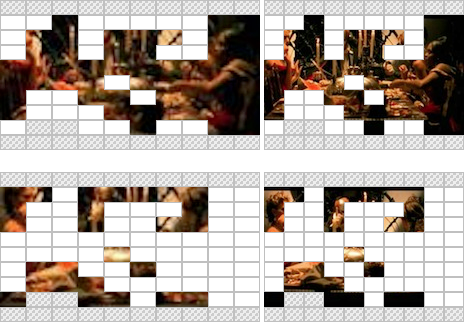
\includegraphics[width=0.75\linewidth]{./similar-different.png}
  \caption[Similar and different corresponding tile pairs]{Similar (upper row) and different (lower row) corresponding tile pairs for the media items from a~Facebook (left column) and a~Google+ user (right column); checkered tiles are not considered due to the black-and-white tolerance}
  \label{fig:similar-different}
\end{figure}

\begin{figure}[!h]
  \centering
  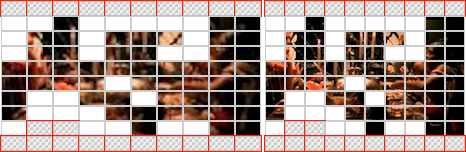
\includegraphics[width=0.75\linewidth]{./tile-highlight.png}
  \caption[Due to the black-and-white tolerance not considered checkered tiles]{Due to the black-and-white tolerance not considered checkered tiles, as the text-to-speech system explains: \textit{``However, 22 tiles were not considered, as they are either too bright or too dark, which is a~common source of clustering issues.''}}
  \label{fig:tile-highlight}
\end{figure}

\subsection{Evaluation}
\label{sec:evaluation}

\paragraph{Evaluating Natural Language Generation Systems:}

For the evaluation of natural language generating systems,
there are three basic techniques.
First, the \emph{task-based} or \emph{extrinsic} evaluation,
where the generated text is given to a~person who evaluates
how well it helps with performing a~given task~\cite{portet2009nlg}.
Second, there are \emph{automatic metrics}
such as BLEU~\cite{papineni2002bleu}, where the generated text
is compared to texts written by people based on the same input data.
Finally, there are \emph{human ratings}, where the generated text
is given to a~person who is asked to rate the quality and usefulness of the text.
For our evaluation, we have chosen the third approach of human ratings,
as we do not evaluate the natural language generating system in isolation,
but in \emph{combination with a~visual representation}
that makes use of spatial Media Fragments URIs
(\autoref{fig:similar-different} and \autoref{fig:tile-highlight}).

\paragraph{Evaluating Subjective Data:}

A~common subjective evaluation technique
is the \emph{Mean Opinion Score} (MOS,~\cite{itu1998mos}).
Traditionally, MOS is used for conducting subjective evaluations
of telephony network transmission quality,
however, more recently, MOS has also found
wider usage in the multimedia community
for evaluating inherently subjective things
like perceived quality from the users' perspective. 
Therefore, a~set of standard subjective tests are conducted,
where a~number of users rate the quality of test samples
with scores ranging from 1 (worst) to 5 (best).
The actual MOS is then the arithmetic mean of all individual scores.

\paragraph{Evaluation Results:}

In the context of this research,
we have conducted MOS test sessions
with five external human raters.
We generated artificially modified deduplicated media item sets
around media items about the \emph{Backstreet Boys}
that were shared on social networks during the time of writing.
These media item sets were curated by yet another independent two external persons,
assisted by a~previously developed software system
that implements the deduplication algorithm described in this chapter.
We asked the two persons to provoke dissent and consent clustering situations
for the five human raters, \emph{i.e.}, obviously correct clustering
(\textbf{Clustering Consent}), obviously incorrect clustering
(\textbf{Clustering Dissent}), and obviously incorrect non-clustering
(\textbf{Non-Clustering Dissent}).
We then asked the five human raters to have the system
automatically explain the algorithm results to them
as described in \autoref{sec:from-debug-output-to-story}.
The raters gave MOS scores ranging from $2$ to $5$,
with the overall average values as follows:
\textbf{Clustering Consent}:~$4.3$, \textbf{Clustering Dissent}:~$3.3$,
and \textbf{Non-Clustering Dissent}:~$4.1$.
The human raters appreciated the parallel explanation approach,
where the visual and the audial parts synchronously described
what the algorithm was doing.
They uttered that the not considered tiles (due to the black-and-white tolerance)
as well as erroneously not detected faces were sources of error
in the algorithm that they easily understood
thanks to the human language description.
They sometimes wished for more diversification in the generated texts.
Without exception, they liked the system and encouraged future development.

\section{Conclusions}

In this chapter, we have treated the topic of media item deduplication
from different angles.
We have first defined the meaning of \emph{exact} and \emph{near-duplicate} 
for both photos and videos,
including the special case of a~photo being contained in a~video.
In a~previous chapter,
we have introduced an algorithm and application
for video shot boundary detection
whose foundations then served for a~more general
photo deduplication algorithm with semantic features
in the present chapter.
We have evaluated the algorithm for two recent events
that had broad social media coverage.
Further, we have outlined how the photo deduplication algorithm
can be used for basic video deduplication,
albeit minimum system response time requirements
hinder its full applicability in practice.
Finally, we have successfully demonstrated the feasibility
of making the task of debugging a~complex algorithm
more human-friendly by means of a~combined visual and audial approach.
We have used Media Fragments URI
together with a~natural language generation framework
realized through a~speech synthesizer to visually and audially
describe media item differences.
The approach was successfully evaluated for its helpfulness and utility
with the evaluation method Mean Opinion Score (MOS).
Our contribution also includes a~polyfill implementation
of spatial Media Fragments URIs.

Media item deduplication of both exact and near-duplicate media items
is a~fundamental step in dealing with huge amounts of social media
and media overload in general.
Highly popular media items not only tend
to retrieve many social interactions on the social network
they were initially shared on, but also on other social networks.
Derivates of popular media items further add noise
to the social media sharing landscape.
Based on our media item deduplication algorithms, 
we have contributed effective and efficient tools
to deal with social media overload
and to identify the few needles in the cross network haystack. 

\section*{Chapter Notes}
This chapter is partly based on the following publications:
\todo{Add publications}

\bibliographystyle{plainnat}
\clearpage
\bibliography{backmatter/references}
